\documentclass[]{usiinfbachelorproject}


%Packages
\captionsetup{labelfont={bf}}



%opening
\title{Spectrally Accurate Resampling of High Quality Rotated Images}
\author{Dylan Reid Ramelli}



\versiondate{\today}

\begin{committee}
	\advisor[Universit\`a della Svizzera Italiana, Switzerland]{Prof}{Rolf}{Krause}
	\assistant[Universit\`a della Svizzera Italiana, Switzerland]{Dr}{Patrick}{Zulian}
	\assistant[Universit\`a della Svizzera Italiana, Switzerland]{Dr}{Diego}{Rossinelli}
\end{committee}

\abstract {
	
}

\begin{document}
	
	\maketitle	
	\section{Introduction}\label{introduction}
	\section{Problem}
	
	
	
	
	\iffalse
	
	\subsection{Interpolation}
	Sampled version of our translated signal is:
	\begin{equation}
		(T_\Delta s)[k] = \sum_{l \in Z}^{} c(l)\varphi(k - \Delta - l)
	\end{equation}
	Where $\varphi$ is our generating function.
	\subsubsection{Linear Interpolation}
	With linear interpolation we want to estimate the coordinates of a point from a given number of samples. 
	
	Linear interpolation model of function sin(x) with $N = 2$:
	\begin{equation}
		\beta^1(x) = 
		\begin{cases}
			1 - |x|, & |x| < 1    \\
			0,       & otherwise, 
		\end{cases}
	\end{equation}
	\begin{center}
		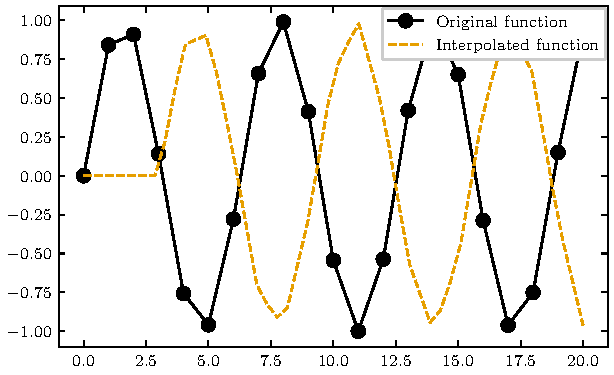
\includegraphics{"images/linear_interpolation_example.pdf"}
	\end{center}
	
	Cubic spline interpolation model of function sin(x) with $N=4$:
	\begin{equation}
		\beta^3(x) = 
		\begin{cases}
			2/3 - |x|^2 + |x|^3/2, & 0 \leq|x| < 1  \\
			(2-|x|)^3/6,           & 1 \leq |x| < 2 \\
			0,                     & 2 \leq |x|     
		\end{cases}
	\end{equation} \cite{main_article}
	
	\begin{center}
		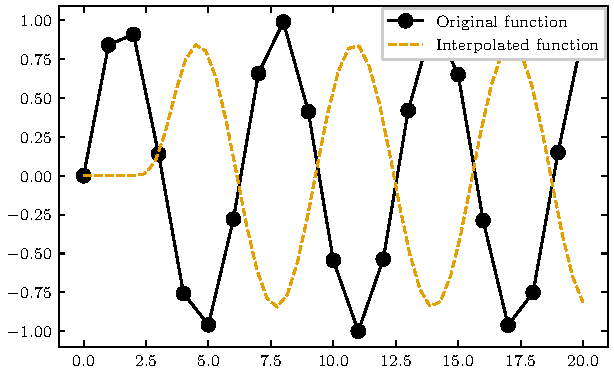
\includegraphics{"images/cubic_interpolation_example.pdf"}
	\end{center}
	
	Standard 2-D interpolation formula for computing the value of the image at location $(x,y)$
	\begin{equation}
		s(x,y) = \sum_{k = k_0}^{k_0+L-1}\sum_{l=l_0}^{l_0+L-1} c(k,l)\varphi(x-k)\varphi(y-l)
	\end{equation}
	
	\fi
	
	
	\section{Solution}
	\section{Validation}
	\section{Conclusion}
	\bibliographystyle{plain}
	\bibliography{references}
	
\end{document}